\documentclass{article}
\usepackage{graphicx}
\begin{document}

\section{que hice}

\begin{itemize}
	\item refactorice
	\item aumento datos
	 \item arregle lo del CE
	 \item datset offline
\end{itemize}

\section{preguntas}

\begin{itemize}
	\item  al hacer el dataset offline, que hacemos con las imagenes en negro?
	\item  dataset offline random vs online
	\item  dev setupp para el ordenador
	\item  de que nos valen imagenes sin mascara
	\item  tanh para lo de la gausiana como lo ve
\end{itemize}
\section{figuras}

\includegraphics[width=\linewidth]{../../data/plots/attention_visualization.png}

\newpage

\includegraphics[width=\linewidth]{../../data/plots/979da3_comparison_plot.png}

\newpage

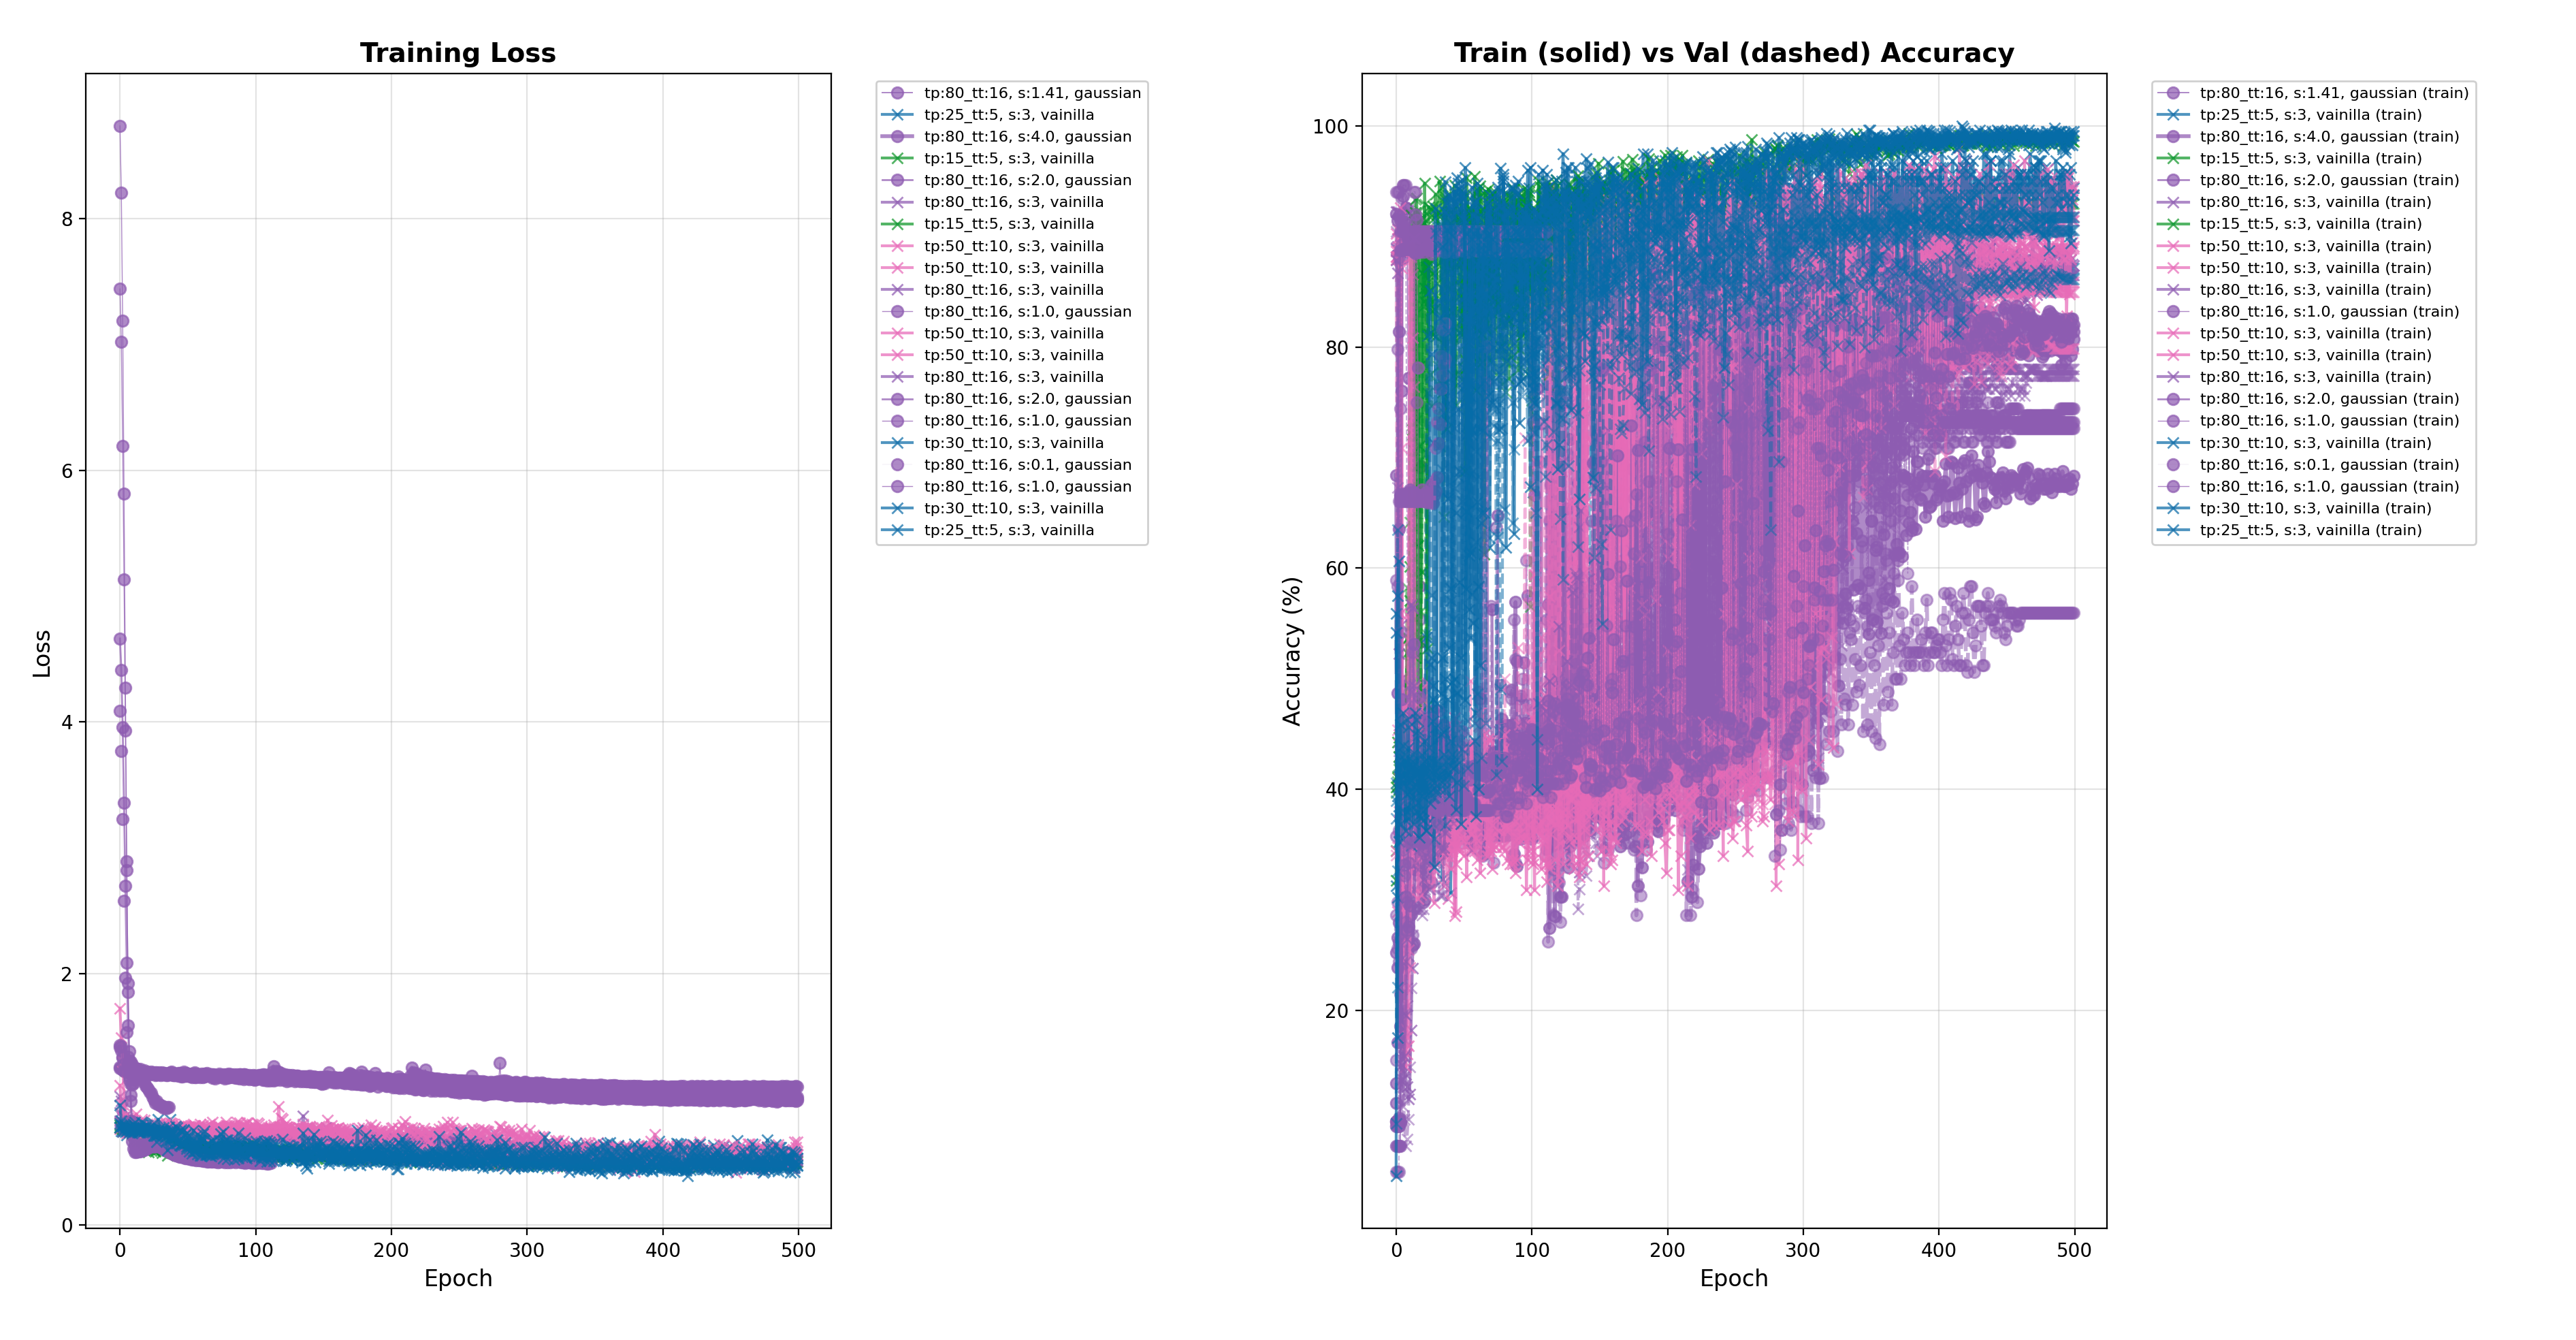
\includegraphics[width=\linewidth]{figs/enorme.png}
\includegraphics[width=\linewidth]{figs/grande.png}
\includegraphics[width=\linewidth]{figs/mediano.png}
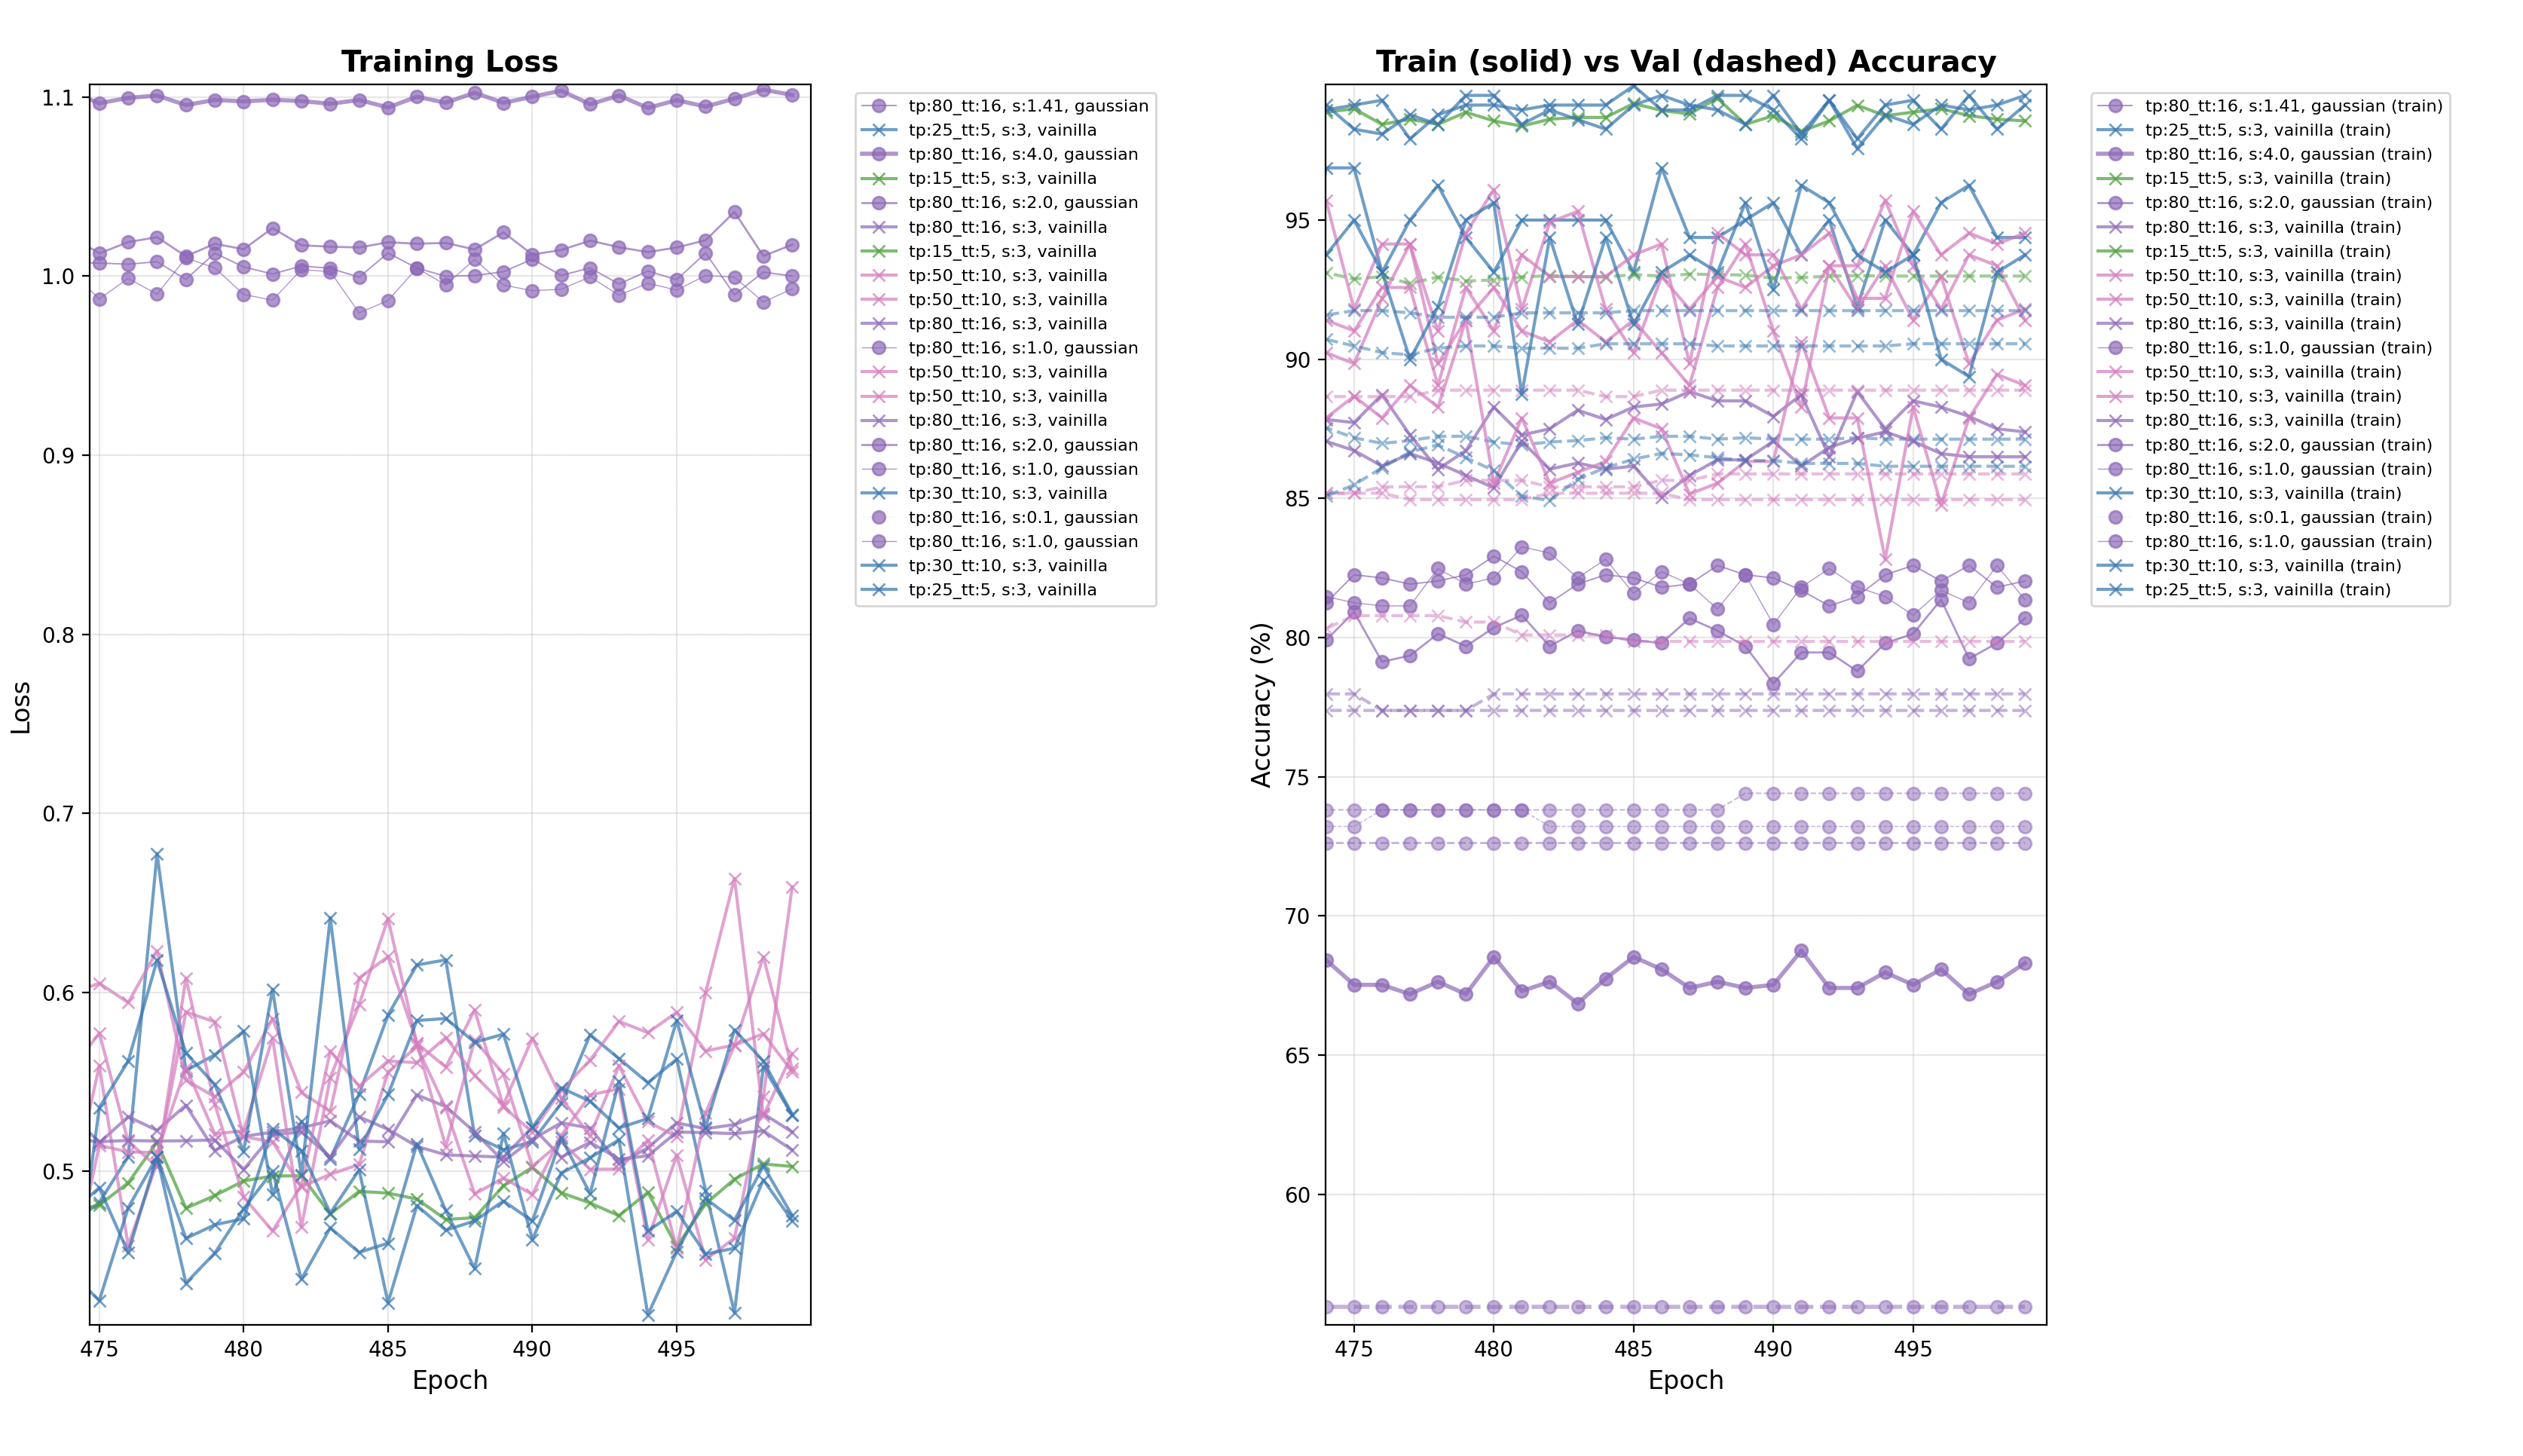
\includegraphics[width=\linewidth]{figs/pequeño.png}

\end{document}
